\chapter{Evaluation}
\label{chapter:evaluation}

\section{Benchmark infrastructure}\label{sec:infra}

We use Caliper as a benchmark tool and HyperLedgerLab to set up the benchmark infrastructure and perform test runs. Modifications to these systems are described in \ref{sec:caliper} and \ref{sec:hll}.

The benchmark runs on an OpenStack cluster and consists of eight instances: three control nodes, three worker nodes, one load-balancer/DNS node, and one node for CLI. The CLI node is not used in the benchmark runs but is employed to set up the infrastructure and orchestrate the runs. Control and worker nodes are of the size m1.large. The rest is m1.medium.

\begin{table}[h!]
\begin{center}
\begin{tabular}{ |c|c|c|c| }
  \hline
  Name & VCPUS & RAM & Disk space \\
  \hline
  \hline
  m1.medium & 2 & 4.88 GB & 10 GB \\
  \hline
  m1.large  & 4 & 9.77 GB & 20 GB \\
  \hline
\end{tabular}
\end{center}
\caption{OpenStack instance flavors}
\label{table:flavors}
\end{table}

\newpage

\section{Benchmark chaincode}\label{sec:benchcode}

We use a simple chaincode with one core transaction to test the new Fabric. The ledger is initialized with one key: "VAR0" and a value 1. The transaction \textbf{moveVar} takes a new key as input, reads the value at "VAR0" and writes it to the new key. By itself,  \textbf{moveVar} is not conflict-free. This property is provided by the benchmark. For each transaction invocation, it picks a random key and invokes \textbf{moveVar} with that key as an argument. This, of course, does not guarantee the conflict-free property but makes transactions practically conflict-free.

\section{Testing plan}\label{sec:testplan}

First, we would like to see how changes in new parameters: batch size and batch timeout affect the throughput. Second, we would like to see if and how the number of peers and the number of organizations influence the throughput. In addition, we expect all or virtually all transactions to be committed. The testing plan is as follows:

\begin{table}[h!]
\begin{center}
\begin{tabular}{ c|c|c|c }
  \# Orgs & peers per org & batch size & batch timeout \\
 \hline
 \hline
 2 & 2 & 30 & 0.3 \\
 \hline
 2 & 2 & 50 & 0.2 \\
 \hline
 2 & 2 & 10 & 0.2 \\
 \hline
 2 & 3 & 50 & 0.2 \\
 \hline
 2 & 4 & 50 & 0.2 \\
 \hline
 3 & 1 & 50 & 0.2 \\
 \hline
 1 & 4 & 50 & 0.2 \\
 \hline
 1 & 3 & 50 & 0.2 \\
 \hline
 1 & 1 & 50 & 0.2 \\
 \hline
\end{tabular}
\end{center}
\caption{Benchmark networks}
\label{table:setups}
\end{table}

Each setup is tested under 100, 200 and 300 TPS with 10000 transactions each. Afterward, a single query transaction is submitted to check if peers respond with consistent results.

\section{Results}\label{sec:testres}

Raw numbers are presented in the Appendix \ref{apdx:fst}. Here we present only the maximal throughput for each scenario and would like to discuss the results in general and what conclusions one can make from them.

\begin{table}[h!]
\begin{center}
\begin{tabular}{ c|c|c|c|c|c|c }
  Setup & \# Orgs & peers per org & batch size & batch timeout & avg latency, s & throughput \\
 \hline
 \hline
 1 & 2 & 2 & 30 & 0.3 & 11.02 & 242.5 \\
 \hline
 2 & 2 & 2 & 50 & 0.2 & 7.97 & 252.4 \\
 \hline
 3 & 2 & 2 & 10 & 0.2 & 9.62 & 252.5 \\
 \hline
 4 & 2 & 3 & 50 & 0.2 & 16.94 & 213.8 \\
 \hline
 5 & 2 & 4 & 50 & 0.2 & 27.35 & 180.7 \\
 \hline
 6 & 3 & 1 & 50 & 0.2 & 10.52 & 247.7 \\
 \hline
 7 & 1 & 4 & 50 & 0.2 & 8.89 & 256.8 \\
 \hline
 8 & 1 & 3 & 50 & 0.2 & 3.52 & 280.3 \\
 \hline
 9 & 1 & 1 & 50 & 0.2 & 0.59 & 297.7 \\
 \hline
\end{tabular}
\end{center}
\caption{Benchmark results}
\label{table:results}
\end{table}

It turns out that under high load the batch size or the batch timeout changes show almost no effect on the throughput. The reason for that lies in the specifics of block processors implementation. Once enough transactions are collected, the block is issued and all clients receive a response, while the block is enqueued to be committed. The benchmark marks a transaction as committed when it receives a receipt, not when the actual block is committed. This approach might pose a problem in an industrial setting but is sufficient for a proof of concept.

Tests have not included the same variability of batch timeouts as with batch size since when testing under high load it becomes virtually irrelevant. When a peer receives more transactions per second than is enough to make a couple of batches, the batch size becomes the limiting factor of the throughput. However it seems to affect the average latency as does the block size.

It is particularly interesting to investigate now the number of peers in the network affects the average latency and the throughput of the network. Relations are illustrated in \ref{fig:avglat1} and \ref{fig:tps1}.

The graphs demonstrate that the throughput drops linearly with the increase in the number of peers. The average latency increases with the increase in the number of peers. These relations show that the current implementation of an orderless system while working perfectly for a small number of peers is not scalable.

Moreover, the number of organizations does not appear to significantly affect throughput. Setups with the same number of peers but a different number of organizations are represented by vertical lines on the graphs at three and four peers. The setup with 2 organizations with 2 peers in each organization, 4 in total, showed essentially the same throughput as the setup with 1 organization with 4 peers in it. This is to be expected since clients have to send the transaction envelope to all peers instead of sending it to one orderer and waiting for block events. It seems that the removal of the bottleneck of the ordering service might increase the throughput but severely hinder the scalability of the system.

However, the scalability issue might be ameliorated by employing anchor peers. Basically, make anchor peer of an organization keep a local ledger, and distribute the blocks of that ledger among the peers of its organization.

This approach has its own downsides. For example, it makes impossible endorsement policies that require endorsements from multiple peers of an organization.

\newpage

\begin{figure}[H]
\begin{center}
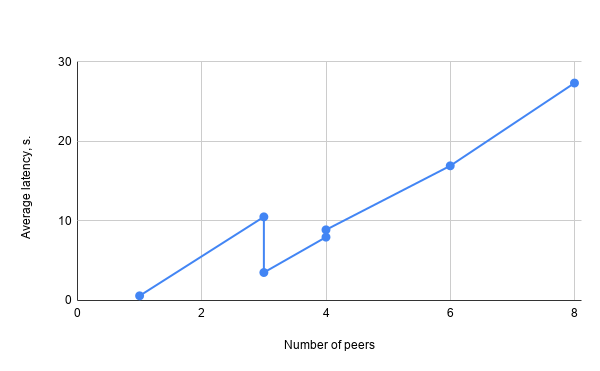
\includegraphics[width=0.75\textwidth]{figures/avglat1}
\end{center}
\caption{Average latency by number of peers. Chaincode 1.}
\label{fig:avglat1}
\end{figure}

\begin{figure}[H]
\begin{center}
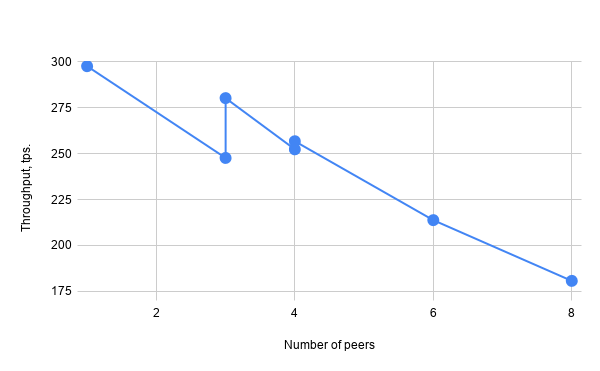
\includegraphics[width=0.75\textwidth]{figures/tps1}
\end{center}
\caption{Throughput by number of peers. Chaincode 1.}
\label{fig:tps1}
\end{figure}

\newpage
\section{Second chaincode} \label{sec:secondchain}

To test whether the system is sensitive to the complexity of the chaincode, we have run the benchmark under the same conditions on a slightly different chaincode.

The principle stays the same: read a value from a fixed key, but instead of simply copying it to a single new location do some extra steps. The value is not copied directly but first unmarshalled to an integer. Then we perform addition on the integer value and write four different results to four distinct keys. This is of course not a very complicated task but if the system is sensitive to the complexity of the transaction this should be enough to manifest in the results of the benchmark.

The throughput and the average latency of the new chaincode for the same network configurations as in \ref{sec:testres} under 300 TPS input are listed in \ref{table:results2}. The raw data is available in \ref{apdx:snd}.

\begin{table}[h!]
\begin{center}
\begin{tabular}{ c|c|c|c|c|c|c }
  Setup & \# Orgs & peers per org & batch size & batch timeout & avg latency, s & throughput \\
 \hline
 \hline
 1 & 2 & 2 & 30 & 0.3 & 10.66 & 252.0 \\
 \hline
 2 & 2 & 2 & 50 & 0.2 & 9.65 & 253.3 \\
 \hline
 3 & 2 & 2 & 10 & 0.2 & 11.59 & 249.3 \\
 \hline
 4 & 2 & 3 & 50 & 0.2 & 9.84 & 250.3 \\
 \hline
 5 & 2 & 4 & 50 & 0.2 & 23.96 & 196.3 \\
 \hline
 6 & 3 & 1 & 50 & 0.2 & 8.94 & 249.5 \\
 \hline
 7 & 1 & 4 & 50 & 0.2 & 8.78 & 256.0 \\
 \hline
 8 & 1 & 3 & 50 & 0.2 & 3.58 & 279.7 \\
 \hline
 9 & 1 & 1 & 50 & 0.2 & 0.64 & 298.1 \\
 \hline
\end{tabular}
\end{center}
\caption{Second benchmark results}
\label{table:results2}
\end{table}

Comparison of the results from the simple and more complicated chaincodes is provided in \ref{table:compare}. Results seem paradoxical. More complex chaincode resulted in increased throughput. However, it might be caused by the fact that in scenarios where there seems to be a paradox some transactions get rejected, which lowers the maximal latency and thus reduces the average latency and slightly increases the throughput.

\begin{table}[h!]
\begin{center}
\begin{tabular}{ c|c|c|c|c|c|c }
  \multirow{2}{*}{Setup} &
  \multicolumn{2}{c|}{Chaincode 1} &
  \multicolumn{2}{c|}{Chaincode 2} &
  \multicolumn{2}{c}{$\Delta_{2 - 1}$} \\ \cline{2-7}
   & avg. lat. & throughput & avg. lat. & throughput & avg. lat. & throughput \\
 \hline
 \hline
 1 & 11.02 & 242.5 & 10.66 & 252 & -0.36 & 9.5 \\
 \hline
 2 & 7.97 & 252.4 & 9.65 & 253.3 & 1.68 & 0.9 \\
 \hline
 3 & 9.62 & 252.5 & 11.59 & 249.3 & 1.97 & -3.2 \\
 \hline
 4 & 16.94 & 213.8 & 9.84 & 250.3 & -7.1 & 36.5 \\
 \hline
 5 & 27.35 & 180.7 & 23.96 & 196.3 & -3.39 & 15.6 \\
 \hline
 6 & 10.52 & 247.7 & 8.94 & 249.5 & -1.58 & 1.8 \\
 \hline
 7 & 8.89 & 256.8 & 8.78 & 256 & -0.11 & -0.8 \\
 \hline
 8 & 3.52 & 280.3 & 3.58 & 279.7 & 0.06 & -0.6 \\
 \hline
 9 & 0.59 & 297.7 & 0.64 & 298.1 & 0.05 & 0.4 \\
 \hline
\end{tabular}
\end{center}
\caption{Comparison of chaincodes}
\label{table:compare}
\end{table}

Average latency and throughput exibit the same behavior in relations to the total number of peers in the network. The throughput decreases and the average latency increases with the increase in the number of peers. See graphs \ref{fig:avglat2} and \ref{fig:tps2}.

Summarizing the compairson, the slight increase in transaction's complexity did not produce significant changes in the performance of the system. However, this comparison can not be considered to be comprehensive because the complexity of the two chaincodes is not different enough. Thus further investigation is required to establish how the system behaves with different sets of transactions.

\begin{figure}[H]
\begin{center}
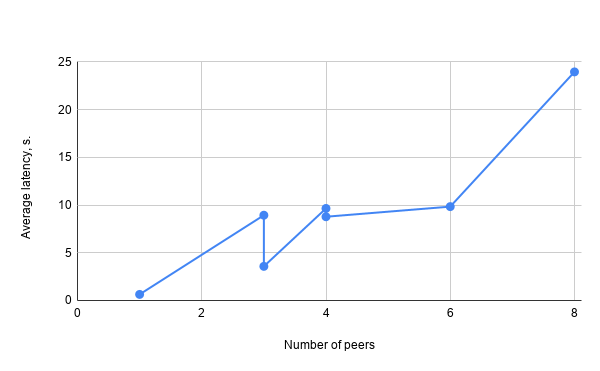
\includegraphics[width=0.75\textwidth]{figures/avglat2}
\end{center}
\caption{Average latency by number of peers. Chaincode 2.}
\label{fig:avglat2}
\end{figure}

\begin{figure}[H]
\begin{center}
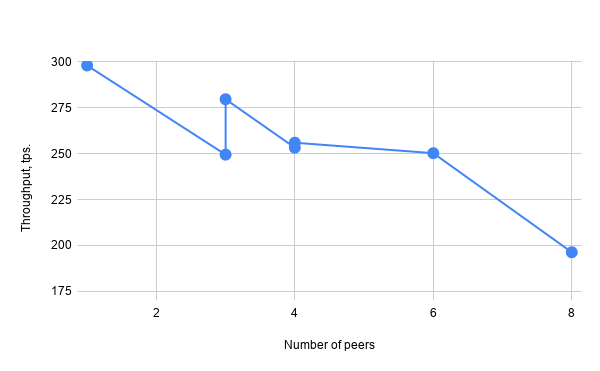
\includegraphics[width=0.75\textwidth]{figures/tps2}
\end{center}
\caption{Throughput by number of peers. Chaincode 2.}
\label{fig:tps2}
\end{figure}
